\documentclass{article}

\usepackage{amsmath}
\usepackage{amssymb}
\usepackage{amsthm}
\usepackage{amssymb}
\usepackage{mathdots}
\usepackage[pdftex]{graphicx}
\usepackage{fancyhdr}
\usepackage[margin=1in]{geometry}
\usepackage{multicol}
\usepackage{bbm}
\usepackage{esint}
\usepackage{listings}
\PassOptionsToPackage{usenames,dvipsnames}{color}  %% Allow color names
\usepackage{pdfpages}
\usepackage{algpseudocode}
\usepackage{tikz}
\usepackage[T1]{fontenc}
\usepackage{inconsolata}
\usepackage{framed}
\usepackage{wasysym}
\usepackage[thinlines]{easytable}
\usepackage{wrapfig}
\usepackage{hyperref}
\usepackage{cancel}
\usepackage{tabu}
\usepackage{tabularx}
\usepackage{mathtools}
\usepackage{mathrsfs}
\usepackage{enumerate}
\usepackage{enumitem}
\usepackage{tabto}

\renewcommand{\P}{\mathbb{P}}
\DeclareMathOperator{\N}{\mathbb{N}}
\DeclareMathOperator{\Z}{\mathbb{Z}}
\DeclareMathOperator{\Q}{\mathbb{Q}}
\DeclareMathOperator{\R}{\mathbb{R}}
\DeclareMathOperator{\C}{\mathbb{C}}
\DeclareMathOperator{\F}{\mathbb{F}}
\DeclareMathOperator{\E}{\mathbb{E}}

% Margins
\topmargin=-0.45in
\evensidemargin=0in
\oddsidemargin=0in
\textwidth=6.5in
\textheight=9.0in
\headsep=0.25in

\title{Implementing and Benchmarking Branch and Bound for Integer Programming: Final Project 6.S098}
\author{Laker Newhouse}
\date{\today}

\begin{document}
\maketitle	

All code and raw results are available at \url{https://github.com/Arongil/6.S098/tree/main/final_project}. \\

\section*{Problem Description}

Linear programming is a surprisingly versatile tool to model countless real-world applications. For instance, it can be used to optimize resource distribution at a hospital (\href{https://pubmed.ncbi.nlm.nih.gov/6232215/}{Brandeau 1984}). However, in the hospital case and in many other applications, it is necessary to force certain variables to be integers. Assigning half a patient to a bed is, sadly, impossible. Most generally this class of problems is called Mixed Integer Programming: some variables are integer, but some remain continuous. In this paper we examine only pure Integer Programming, in which all variables are constrained to be integers. The purpose of this paper is to describe an implementation for an algorithm called branch and bound which solves integer programs. Naive iteration takes exponential time in the input; branch and bound seeks to set lower and upper bounds to prune large swaths of the search tree.

A number of techniques to speed up branch and bound have been studied (\href{https://digitalcommons.usu.edu/cgi/viewcontent.cgi?article=2179&context=gradreports}{Wu 1973}, \href{https://www.researchgate.net/publication/257588965_Speeding_up_branch_and_bound_algorithms_for_solving_the_maximum_clique_problem}{Maslov, Batsyn, Pardalos 2014}). Domain specific speed ups are also typically achievable. Our algorithm does not implement these speed ups. As a result, the solver does not work on large, real world problems. For this reason we have chosen to develop a modestly sized, synthetic dataset for the purpose of benchmarking, recognizing that to solve any large, real world application with our implementation would require extensive speed ups. We chose to benchmark on bin packing. Finally, we compare our results against the time taken by one of the fastest non-commercial and open-source integer programming solvers, \href{https://www.scipopt.org/}{SCIP}.

\section*{Branch and Bound}

The standard form of an integer program is as follows: \begin{align*}
    \text{maximize } & c^T x \\ 
    \text{subject to } & Ax \leq b \\
    & x \geq 0 \\
    & x \text{ integer}.
\end{align*} The naive way to solve an integer program would be to enumerate all possible integer solutions to $x$ and check them one by one. This does not work if the feasible region is unbounded, and anyway it would be enormously slow.

A key idea in what follows is relaxation, which is when we remove the constraint that $x$ must have integer values. A relaxed integer program is a regular linear program. We know how to solve those. We can obtain the optimal solution $x^\ast$ to the relaxed problem almost instantly. If we are lucky, this solution will happen to be integer already. If so, we are done. Otherwise, it will have some fractional entries.

In the branch and bound algorithm, we select one such fractional entry. Say the $i^\text{th}$ entry of $x^\ast$ is $4.2$. Obviously we cannot allow this. What we can say, however, is that the true optimal solution will have either $x_i \geq 5$ or $x_i \leq 4$. This is the key idea.

We construct two new integer programs: one adds the constraint $x_i <= \lfloor x_i^\ast \rfloor$ while the other adds the constraint $x_i >= \lceil x_i^\ast \rceil$. We then apply branch and bound to each of these linear programs.

The result is a binary tree of integer programs. Each is solved in turn by relaxing the integer constraint, finding the optimal relaxed solution, checking whether it is already integer, and if not adding two more problems to the list with inequalities forcing one more fractional entry to become linear. Whenever we find an all-integer solution, we note down the objective function value is produces. We save this as a lower bound $l$.

Notice, however, that whenever we solve the associated relaxed linear program, we find an upper bound on how well the integer solution could do. The integer solution, after all, can only be more constrained than the relaxed version. But we also know we can do at least as well as $l$. Therefore, if the constraints that led to this subproblem make the relaxed version do more poorly than even $l$, there is no hope for this branch. Further constraints will only further deteriorate performance. Therefore we can prune a branch whenever its relaxed optimal is worse than our current best all-integer optimal.

The idea behind branch and bound is to constantly keep track of a minimum attainable objective value. The algorithm takes advantage of this lower bound to prune large swaths of the search tree, saving sometimes trillions of explorations further down the line. In our implementation, we use a queue which stores subproblems. The algorithm picks one at a time to investigate, either pruning or adding more children on to the queue to explore. Empirically, we determined that a LIFO queue is faster than a FIFO queue.

Several heuristics exist to decide which fractional entry to branch on. We apply one of the simplest such heuristics, which is to branch on the most infeasible entry, meaning the entry whose decimal part is closest to $0.5$. We saw performance gains over naively selecting the first fractional entry as the branch point.

We repeat that the full code for our implementation is available at \url{https://github.com/Arongil/6.S098/tree/main/final_project}.

\section*{Benchmarking the Algorithm}

We benchmark the branch and bound algorithm on the bin packing problem, which goes as follows.

We have $n$ objects with integer weights from $1$ to $100$. We have unlimited bins in which to place them, but we wish to minimize how many bins we use. Furthermore, each bin can hold at most weight $100$. How should we place the objects so as to achieve our objective of using the fewest bins?

We formulate the bin packing problem using $n^2 + n$ variables and $3n$ constraints. This rests on the observation that we will need no more than $n$ bins. The first $n^2$ variables $x_{ij}$ represent whether object $i$ is in bin $j$. The final $n$ variables represent whether bin $j$ is used. These variables are binary. The first $2n$ constraints ensure that each item is in exactly one bin. We need twice the constraints because two inequality constraints go in to form each equality constraint. The final $n$ constraints ensure that no bin is packed beyond its capacity.

We encode the variables as an $n^2 + n \times 1$ vector $x$ and the constraints as an inequality $Ax \leq b$, for a $3n \times 1$ vector $b$ and a $3n \times n^2 + n$ matrix $A$. The matrix can end up with many, many entries and is extremely sparse. We do not take advantage of the sparsity but recognize that this would constitute a future direction for speed ups.

We graph the benchmark results below for different values of $n$, with milliseconds on the $y$ axis.

\begin{center}
    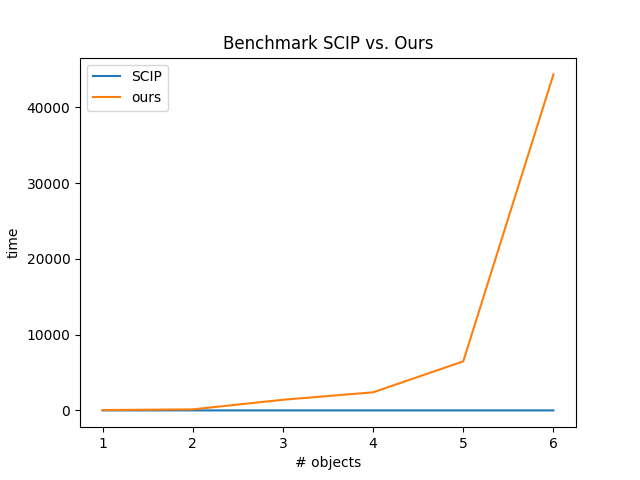
\includegraphics[scale=0.5]{benchmark_no_target}
\end{center}

We observe SCIP performs almost linearly, taking about $n$ milliseconds per problem. Almost immediately, however, the exponential nature of the problem hampers our algorithm. The most probable issue is that branch and bound is simply not very effective in the bin packing problem: there is not enough opportunity to prune. For example, the best solution may involve $12$ bins. The problem may find a solution with $12$ bins in the first few seconds, but nonetheless press on lest it miss a superior option. In most integer programming scenarios there is more fine grain variation in the objective function which could allow further pruning.

To compensate, we make one common sense speed up which is to allow branch and bound to halt if it reaches some chosen target numbers of bins. We do not sacrifice on finding the global optimum if we choose this target well. We choose it to be the smallest integer greater than the summed weights of all objects, divided by $100$. As one can see, it is impossible to fit weights of $99$, $98$, $97$, and $3$ into fewer than $3$ bins because the total weight exceeds $200$. If such a solution is found, we therefore mark it as optimal and stop the search.

The graph below shows how such a simple extra rule can yield massive performance gains. Nonetheless, the algorithm again falters as soon as the target is less than the true minimum number of bins. After all, the target is a best case.

\begin{center}
    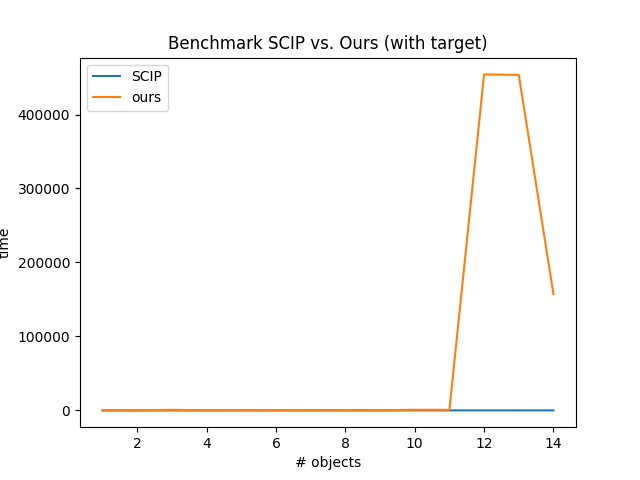
\includegraphics[scale=0.5]{benchmark_yes_target}
\end{center}

Here we observe a funny phenomenon. If the solver gets lucky, as often occurs for low values of $n$, then it can often come to its target number of bins within seconds. If not, it falls down the exponential rabbit hole. Further optimizations like this one layered atop one another could bring the solve time of our homemade algorithm down to a level comparable with modern, open-source solvers.

\section*{Conclusion}

The strength of convex optimization is its wide applicabilty and its blazing speed. Indeed, to solve a single integer program requires solving often thousands of linear programs, and yet still the process can finish in seconds. Convex optimization may not, however, be the best way to approach the bin packing problem. For example, one can formulate a polynomial time algorithm which achieves within $1$ of the optimal solution (\href{sciencedirect.com/science/article/abs/pii/S0377221706004310?via\%3Dihub}{Filippi}). Nevertheless, bin packing serves well as a benchmark for the branch and bound algorithm.

While branch and bound is an effective technique to prune the search tree in integer programs, the data bears out our conclusion that it is not enough alone to solve more than quite modestly sized real-world problems. Further improvements such as cutting plane inequalities could help. There is a literature on such optimizations.

We feel it has been an excellent learning experience to implement branch and bound. Certainly it reinforces a sense of wonderment and gratitude for the work of optimization scientists come before us. They have explored high peaks and endless passageways to build solvers -- many open source -- which measured on average time are complexity classes better than our mostly naive solution.

Lastly, we thank Alex Amice and Benoit Legat for a lively course in which we have learned much.

\end{document}
